\section{Design} \label{sec:design}

This section describes the requirements of the database, and how the Entity 
Relation diagram was designed to facilitate those requirements. 

\subsection{Requirements}

We want our database to be compatible for storing train systems and planning 
routes. Therefore we want parts of our database relations to easily resemble 
graph structures. These ``graph'' relations are specifically \emph{Station}, 
\emph{Route}, \emph{Track}, and \emph{RouteTracks}.\\
That is, \emph{Station} can be seen as the relation containing vertices, and \emph{Track} containing the edges between vertices. \emph{RouteTracks} then contains a composition of tracks/edges to resemble a route that connects through different stations/vertices.\\[12pt]
The other relations like \emph{Train}, \emph{Employees} and \emph{Shift} are 
not really key parts of our database functionality, but are relations that 
should be included none the less.

% Functional requirements:
% Views:
%  * Length of a route
%  * View stations on a route
% Functions / Triggers / ... Mention functionality of those (NOT how they were 
% implemented)

\subsection{ER diagram}
Figure~\ref{fig:ER} shows our ER diagram, which illustrates the design of our 
\emph{Train Management} schema. It shows that some entities have total 
participation in some of the relations, as for instance you cannot have tracks 
without stations or cities, neither can you have routes without tracks.

\newpage
\begin{figure}[ht!]
    \centering
    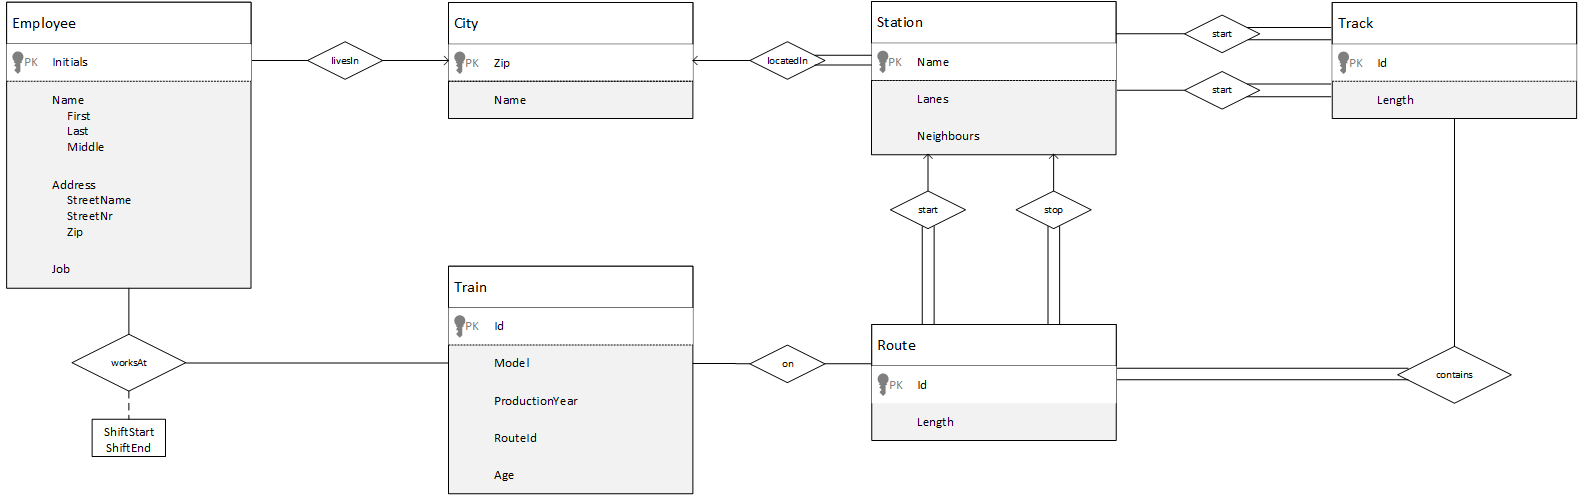
\includegraphics[angle=90,origin=c,width=.4\textwidth]{img/Handwritten_ER}
    \caption{An ER diagram depiction the design of the database}
    \label{fig:ER}
\end{figure}

% Design coices 
% See notes on hand drawn ER diagram (marked by *) None of those 3 examples 
% have been mentioned

% Comments on ER diagram supporting the requirements
